\subsection*{۱.۱}

در ابتدا، DFA این زبان را رسم می‌کنیم. برای این‌که از هرگونه اشتباهی جلوگیری کنیم، پرانتز باز "(" را با a نشان می‌دهیم و پرانتز بسته ")" را با b نشان می‌دهیم. چون هیچ پرانتز باز و بسته ای وجود ندارد یا در واقع تعداد هر دو 0 است، به عنوان accept state آن‌ها را می‌پذیریم. در استیت اولیه، با دیدن پرانتز بسته به حالت trap رفته و با دیدن پرانتز باز، به استیت بعدی می‌رویم. همچنین در استیت‌های بعدی، با دیدن پرانتز بسته به استیت قبلی رفته و با دیدن پرانتز باز به حالت بعدی می‌رویم. همچنین اگر تعداد پرانتزهای باز بسته نشده به بیش از 4 عدد برسد، به حالت trap می‌رویم. همچنین همان استیت اولیه‌ی ما، استیت accept می‌باشد.

\begin{center}
	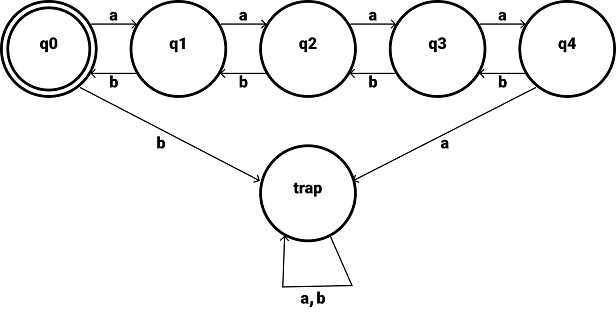
\includegraphics{DFA11}
\end{center}

حالا برای تبدیل آن به عبارات منظم، باید به شکلی از GNFA در آوریم آن را. در نتیجه باید یال ورودی به استیت ۰ و یال خروجی از استیت پایانی نداشته باشیم. همچنین این ۲ استیت باید متفاوت باشند و مثل DFA کشیده شده نباید یکسان باشند. برای این‌کار، استیت s را به عنوان استیت شروع اضافه می‌کنیم به DFA کشیده شده و از استیت پایانی آن را جدا می‌کنیم. از استیت s به استیت شروع قبلی یک یال اپسیلون اضافه می‌کنیم. همچنین استیت f اضافه می‌کنیم به DFA و از استیت پایان قبلی یک یال اپسیلون به آن اضافه می‌کنیم. حالا بین هر ۲ حالتی که یال نداریم باید یال‌های تهی اضافه کنیم. (این یال‌ها در عکس پایین نشان داده نشده‌اند ولی) 


در نتیجه الان استیت شروع و پایان جدیدی داریم که یکسان نیستند و یال ورودی به استیت شروع و یال خروجی از استیت پایانی نداریم.

\begin{center}
	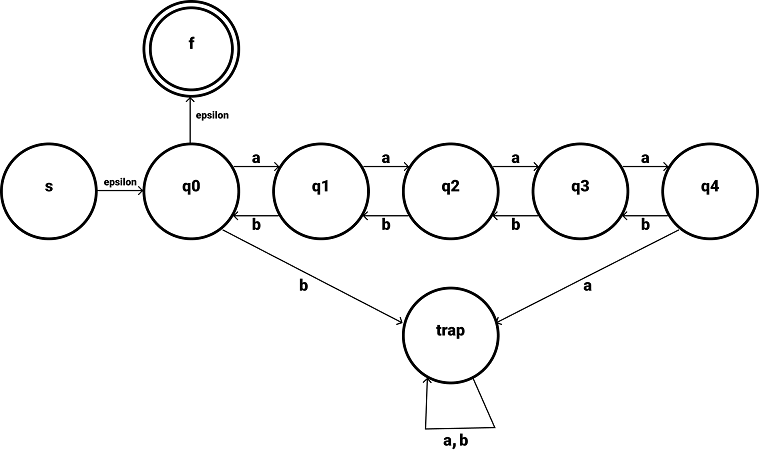
\includegraphics{DFA12}
\end{center}

حالا مرحله به مرحله به حذف یال‌ها می‌پردازیم و GNFA را آپدیت می‌کنیم. با توجه به این‌که حالت trap فقط به خودش یالِ غیر از تهی دارد، با حذف آن تغییری در باقی استیت‌ها و سایر یال‌ها رخ نمی‌دهد و چون concat یک string با Ø، خود Ø می‌شود، تغییری به طور کلی ایجاد نمی‌شود با حذف آن.

\begin{center}
	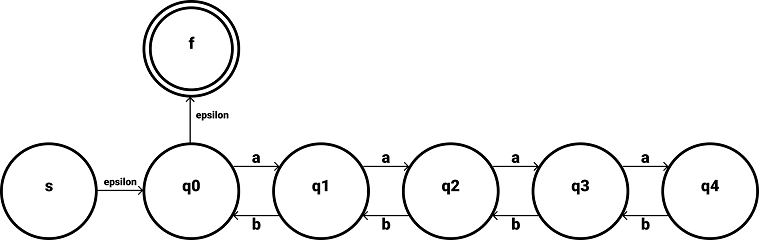
\includegraphics{DFA13}
\end{center}

حالا به ترتیب، به حذف استیت‌های ۴، ۳، ۲، ۱ و ۰ می‌پردازیم تا فقط استیت‌های s و f باقی بمانند. برای هر کدوم از آن‌ها بررسی می‌کنیم که چه یال‌های غیرتهی دارند به دیگر استیت‌ها و مطابق الگوریتم گفته شده، به خودشان وصل می‌کنیم استیت‌های قبلی استیت‌های حذف شده را و به ترتیب که این‌کار را انجام دهیم، DFA مدنظر ما بدست می‌آید.
در نهایت با توجه به این روش و روند حل، در نهایت عبارت منظم خواسته شده به شکل 
$$ (a(a(a(ab)*b)*b)*b)*$$
می‌باشد.

\begin{center}
	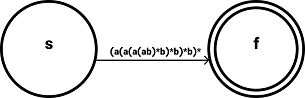
\includegraphics{DFA14}
\end{center}

دلیل درستی این DFA این است که به ازای هر ورودی پرانتز می‌بایست یک ورودی پرانتز بسته یا y دریافت کنیم که به استیت‌های قبلی و در آخر به استیت شروع که حالت accept ما می‌باشد، برویم. همچنین اگر عمق بیش از ۴ شود، به استیت trap می‌رویم و در آن می‌مانیم همیشه.



\subsection*{۲.۱}

در بخش دوم از سوال ۱، تابع stammer به صورت بازگشتی تعریف شده است و هر حرف رشته‌ی ورودی خودش را، دو بار تکرار می‌کند. برای مثال در صورتی که ورودی آن
$w_1 w_2 ... w_n$
باشد، خروجی آن
$w_1 w_1  w_2 w_2 ... w_n w_n $
خواهد بود. حالا دستگاهی را در نظر می‌گیریم که زبان L را می‌شناسد؛ می‌توان دستگاه جدیدی ساخت که زبان
$stammer^-1 (L)$
را بشناسد. 	برای این دستگاه خواهیم داشت

زبان L :
$$M = (Q, \Sigma, \delta, q, F)$$
زبان 
$stammer^-1 (L)$
$$N = (Q, \Sigma, \delta_2, q, F)$$
برای قواعد زبان
$stammer^-1 (L)$
داریم که 
$$\delta_2 (q, a) = \delta (\delta (q, a), a)$$
پس این ماشین می‌تواند زبان مدنظر را شناسایی کند و اگر در ماشین ابتدایی ورودی 
$w_1 w_1  w_2 w_2 ... w_n w_n $
داشته باشیم، از استیت‌های 
$q_1 q_2 ... q_n $
عبور می‌کند و در ماشین جدید، رشته‌ی
$w_1 w_2 ... w_n$
از استیت‌های فرد یعنی
$q_1 q_3 q_5 ...$
عبور می‌کند.
پس چون توانستیم برای این زبان، DFA طراحی کنیم، این زبان منظم است.

\subsection*{۳.۱}

در این بخش از یک سمت تساوی شروع می‌کنیم و به سمت دیگر می‌رسیم.
$$(xy^{*}z)^{*}(xyz(xy^{*}z)^{*})^{*} = (xy^{*}z \cup xyz)^{*}, \quad \text{با توجه به همانی پایه} \, (xy^{*}z)^{*} = (x \cup y)^{*}$$
$$ = (x(y^{*} \cup y)z)^{*}, \quad \text{با توجه به همانی پایه} \, L(M \cup N) = LM \cup LN,\,(M \cup N) L = ML \cup MN$$
$$ = (xy^{*}z)^{*}, \quad \text{با توجه به} \, y^{*} = (y^{*} \cup y)$$


با توجه به این‌که اجتماع رشته
$y$
و
$y^{*}$
می‌شود
$y^{*}$
، چون که از صفر یا بیشتر
$y$
تشکیل شده است.

برای قسمت بعدی هم ابتدا نشان می‌دهیم.
$$(x \cup y)^{*} = x^{*}(yx^{*})^{*}$$
می‌دانیم رشته
$x^{*}(yx^{*})^{*}$
زیرمجموعه‌ی رشته
$(x \cup y)^{*}$
است زیرا که تنها می‌تواند از حروف
$x$
و
$y$
تشکیل شده باشد. همچنین می‌دانیم
$(x \cup y)^{*}$
زیرمجموعه
$x^{*}(yx^{*})^{*}$
است چرا که برای هر رشته متشکل از تعدادی
$x$
و
$y$
دلخواه از شمردن
$x$
شروع می‌کنیم و هرجا
$y$
بود،
$yx^{*}$
را قرار می‌دهیم و تا انتها پیش می‌بریم. به این ترتیب هر رشته متشکل از این دو حرف در عبارت
$x^{*}(yx^{*})^{*}$
وجود خواهند داشت پس داریم.
$$(x \cup y)^{*} = x^{*}(yx^{*})^{*}$$

برای حالت 
$(x \cup y)^{*} = x^{*}(x^{*} y)^{*}$
نیز به همین صورت خواهد بود با این تفاوت که این بار می‌توان از آخر رشته شروع کرد و هر
$y$
دیدیم به همراه رشته
$x$
به دنبال آن عبارت
$x^{*} y$
را قرار دهیم. در نتیجه بدست می‌آوریم که:
$$(x \cup y)^{*} = x^{*}(x^{*} y)^{*} = x^{*}(yx^{*})^{*}$$